
\begin{figure}[h!]
    \centering
    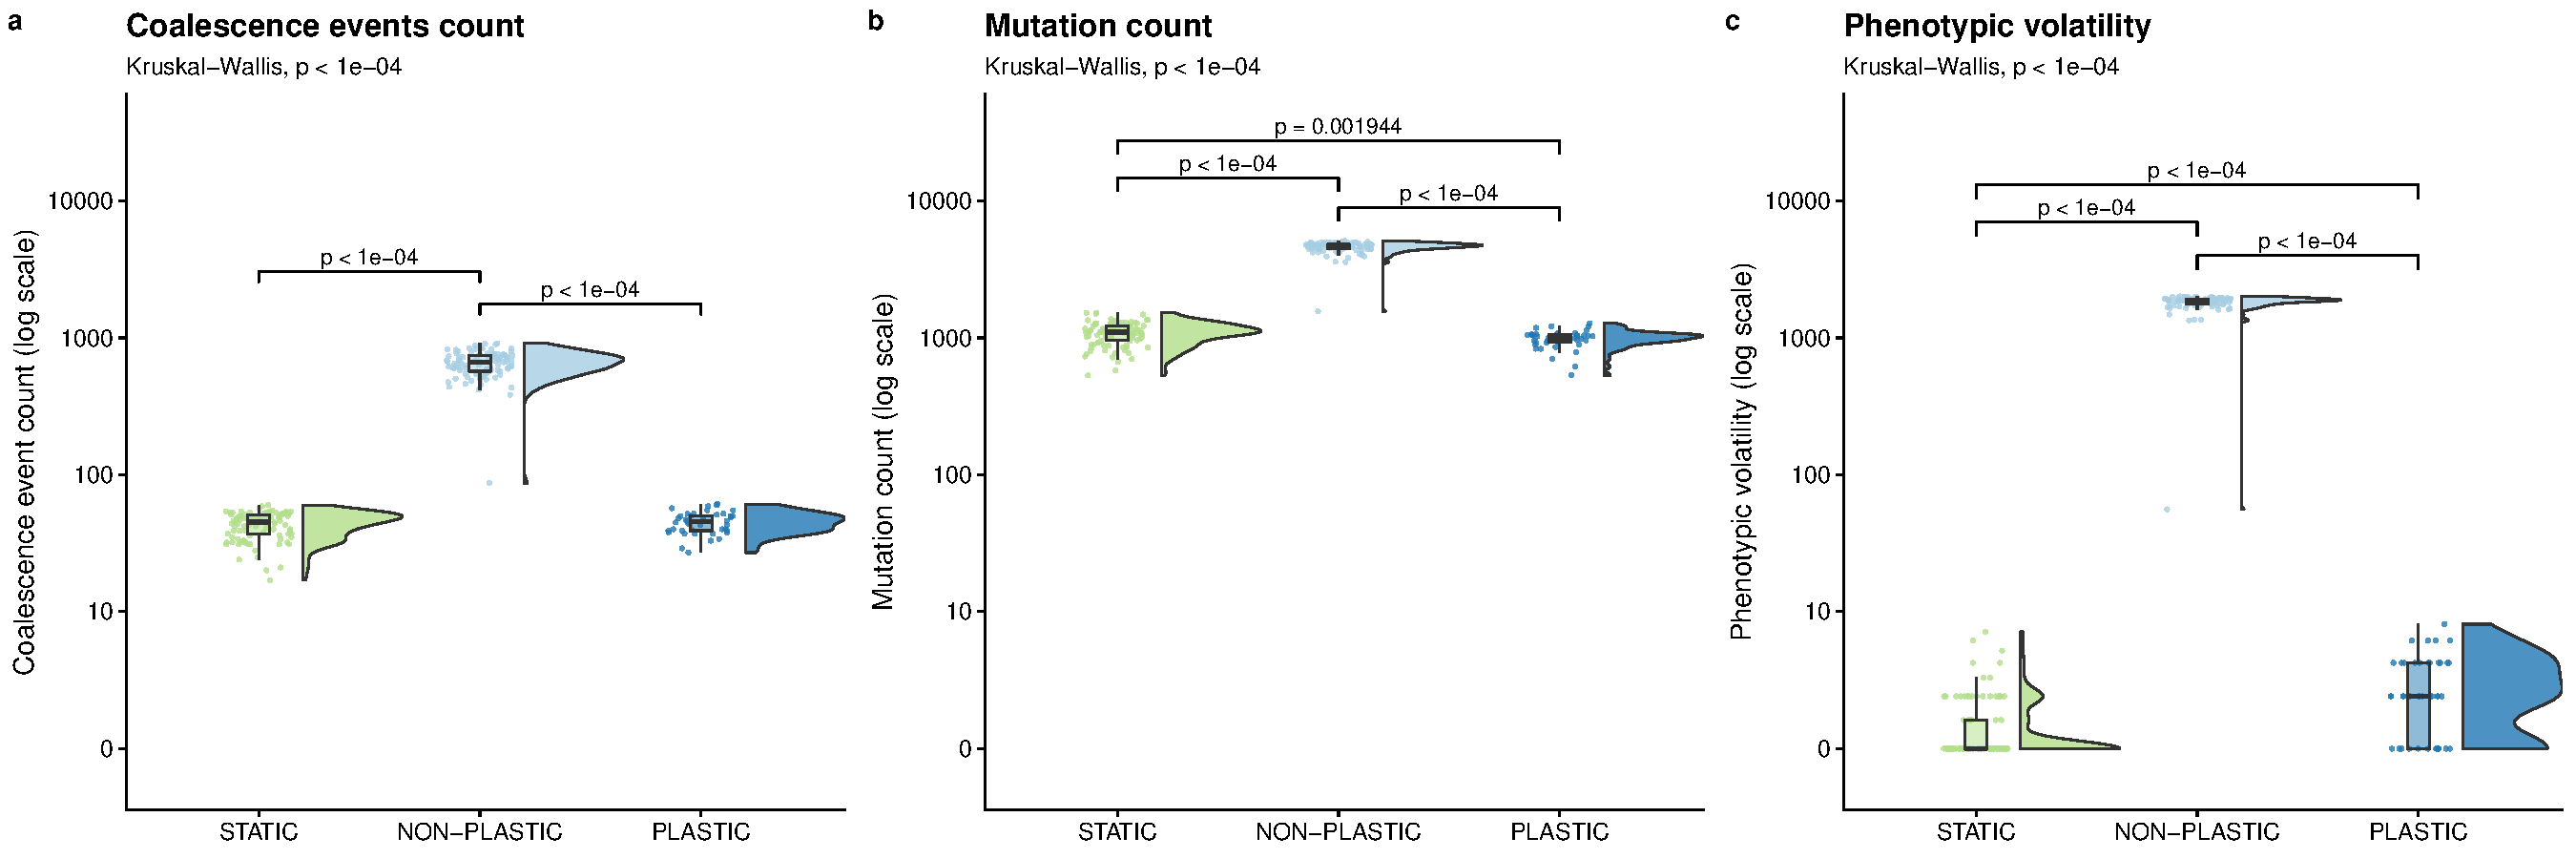
\includegraphics[width=1\textwidth]{media/evolutionary-change-magnitude-panel.pdf}
    \caption{\small
    \textbf{Magnitude of evolutionary change.}
    Raincloud plots \citep{allen_raincloud_2019} of 
    (a) coalescence event count, 
    (b) mutation count, 
    and (c) phenotypic volatility. 
    See Table \ref{tab:metrics-definitions} for descriptions of each metric.
    Each plot is annotated with statistically significant comparisons (Bonferroni-corrected pairwise Wilcoxon rank-sum tests).
    Note that adaptive phenotypic plasticity evolved in \evolutionaryChangeRatePlasticReps\ of \evolutionaryChangeRateReplicates\ replicates from the PLASTIC treatment during phase one of this experiment; we used this more limited group to found \evolutionaryChangeRatePlasticReps\ phase-two PLASTIC replicates from which we report these PLASTIC data.
    }
    \label{fig:evolutionary-dynamics-magnitude}
\end{figure}